

\chapter{Grundlagen}

\section{Einführung)}
Im Gegensatz zu weiten Teilen der Informatik besteht in der Telekommunikation seit langem die Notwendigkeit,
herstellerunabhangige und präzise Standards für Kommu- nikationsprotokolle und -dienste zu erstellen. Diese Anforderung hat dazu gefuhrt, dass man sich schon frühzeitig mit der Entwicklung der formalen Modellierungssprachen Message Sequence Chart (MSC) und Specification and Description Language (SDL) beschaftigt hat. Im Gegensatz etwa zur Unified Modeling Language (UML) liegt MSC
und SDL eine formale Semantik zugrunde, die die Bedeutung der einzelnen Sprachkonstrukte klar und eindeutig
definiert.\\
MSC und SDL sind von der International Telecommunication Union standardisiert worden. Fur beide Sprachen existieren eine graphische Reprasentation (MSC /GR bzw. SDL/GR) fur die Benutzung durch Menschen und eine textuelle Notation (MSC/PR bzw. SDL/PR) fur eine maschinelle Weiterbearbeitung. MSC und SDL werden haufig gemeinsam im Software-Entwicklungsprozess eingesetzt. MSC dient dabei zur Anforderungsdefinition, Testfallspezifikation und Dokumentation, wahrend SDL in der Spezifikationsphase und der Implementierungsphase eingesetzt wird.

\section{Unified Modeling Language (UML)}

\subsection{Historie und Ziel}
Die Unified Modeling Language (UML) ist eine durchgängige Modellierungssprache von der
organisatorischen Beschreibung von Geschäftsprozessen bis zu direkt ausführbaren Modellen,
d.h. bis zur Implementierung. Sie ist über ISO standardisiert (ISO /IC 19501).\\
Ein erster Ansatz wurde 1990 auf der Grundlage verschiedener Notationssysteme entwickelt.
Die Standardisierung, Pflege und Weiterentwicklung der Sprache wurde an die OMG
übergeben, die die Sprache im Jahr 1997 zur Version UML 1.1 weiterentwickelte. Seit Ende der
1990er Jahre haben zahlreiche Personen und Institutionen intensiv an der UML Version 2.0
gearbeitet, die im Jahr 2006 vollständig fertig gestellt und Anfang 2009 von der leicht
überarbeiteten Version 2.2 abgelöst wurde. Eine Standardisierung durch die International
Standardization Organization (ISO) hat die Version 2.2 allerdings noch nicht erreicht. Diese
bleibt bisher nur der Version 1.4.2 vorbehalten.

\subsection{Metamodell}
UML legt Spracheinheiten fest, die auf verschiedenen Ebenen agieren. Mit diesen drücken Sie die Struktur und das Verhalten eines Systems aus. Einige Elemente nutzt die Modellierungssprache, um sich selbst zu definieren. Die Meta-Modellierung umfasst alle Elemente von UML, auch solche, die UML selbst beschreiben. Dafür nutzt es vier hierarchisch angeordnete Ebenen (M0 bis M3).\\

Die Meta-Metaebene M3 spezifiziert die Metadaten der Modellierungssprache und deren Zusammenhänge mithilfe der Meta Object Facility (MOF). Sie definiert das Metamodell. Zudem befähigt Sie den Metadaten-Transfer. Das von der OMG definierte Format XMI ist ein praktisches Tool, um objektorientierte Daten auf Meta-Metaebene zwischen Entwicklungstools zu teilen. Die Object Constraint Language (OCL), eine deklarative Programmiersprache, ergänzt UML und reguliert Randbedingungen der jeweiligen Modellierung. Als Textsprache wirkt sie jedoch nur unterstützend, statt selbst für Modellierung zur Verfügung zu stehen.\\

\begin{center}
\begin{figure}[h]
   
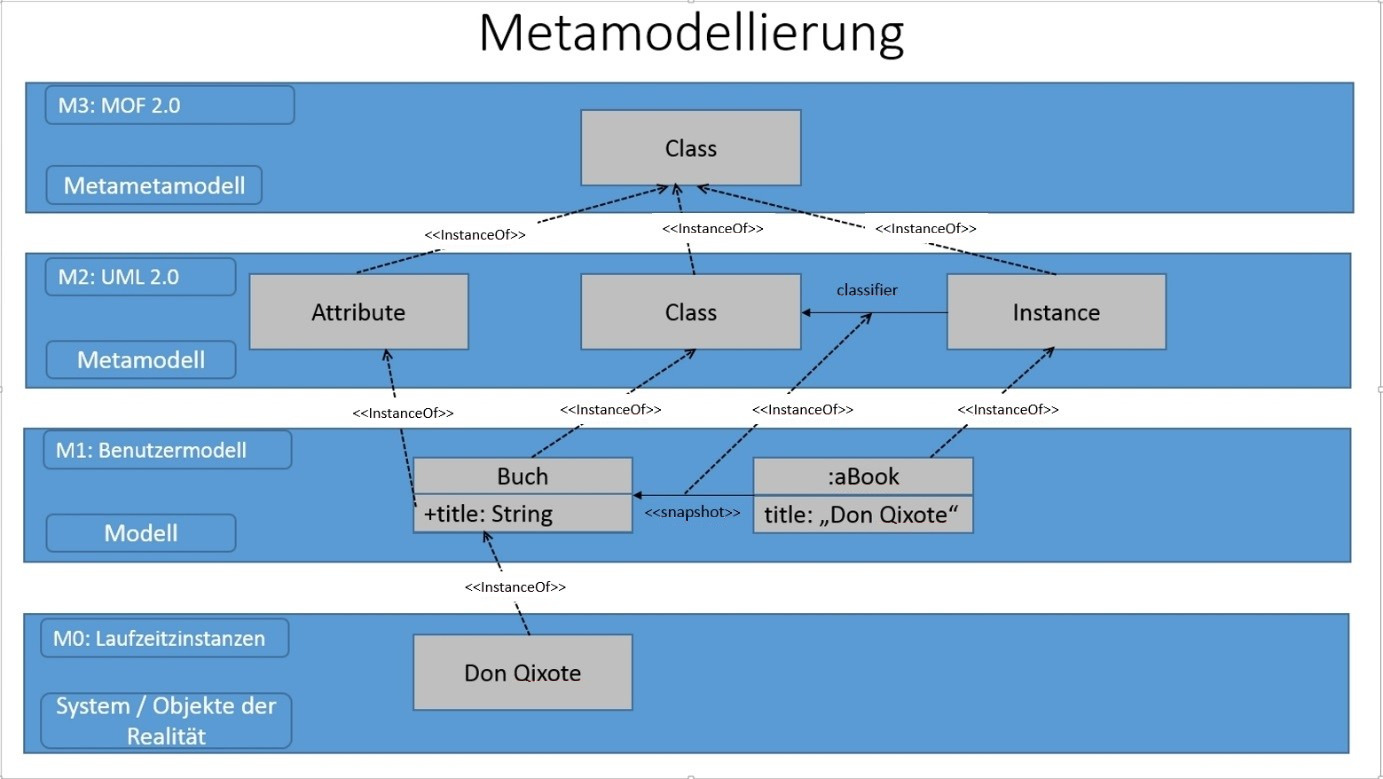
\includegraphics[scale=1]{Graphics/metamodell.jpg} 
\captionof{figure}{Die Metamodellierung zeigt die hierarchische Beziehung zwischen den Sprachebenen}



Quelle : Ionos - Digital Guide

\label{fig1}


\end{figure}
\end{center}
\newpage

Die obere Grafik zeigt die Metamodellierung von UML 2.0. Ebene M0 ist die grundlegende Ebene. Sie stellt konkrete, reale Objekte und einzelne Datensätze dar – z. B. ein Objekt oder eine Komponente. Ebene M1 umfasst alle Modelle, die die Daten der Ebene M0 beschreiben und strukturieren. Das sind UML-Diagramme wie das Aktivitätsdiagramm oder das Paketdiagramm (weiter unten erklärt). Um den Aufbau dieser Modelle zu definieren, legen Metamodelle der Ebene M2 die Spezifikationen und Semantik der Modellelemente fest.\\

Wollen Sie ein verständliches UML-Diagramm erstellen, müssen Sie das Metamodell UML mit seinen Regeln kennen. Die höchste Ebene, M3, ist ein Metamodell des Metamodells. Die erwähnte Meta Object Facility arbeitet auf einer abstrakten Ebene, die Metamodelle definiert. Diese Ebene definiert sich selbst, da sonst weitere, übergeordnete Meta-Ebenen entstünden.\\

\subsection{Kurzbeschreibung}
Bei der Unified Modeling Language (UML) handelt es sich nicht um eine bestimmte Methode, sondern vielmehr um einen Sammelbegriff für grafische Methoden der objektorientierten Entwicklung und Dokumentation von Software (Object Oriented Design – OOD). Dies umfasst Methoden und Notationen für Planung, Design, Entwurf und Implementierung von Software, die seit den 90er Jahren durch die Object Management Group (die auch BPMN pflegt) zu einem offiziellen Standard, der UML, zusammengeführt wurden.\\
Im Gegensatz zu anderen Methoden, die primär auf die Modellierung von Prozessen abzielen, kann die UML direkt zur Software-Entwicklung genutzt werden.\\
Die objektorientierte Sichtweise, auf der UML basiert, zieht ausgehend von der realen Welt Objekte heraus, die mit Attributen beschrieben werden. Die Objekte werden zu Klassen verdichtet, wenn Eigenschaften und Verhalten der Objekte identisch oder ähnlich sind. Klassen können daher als Baupläne für die zu erzeugenden Objekte (die Instanzen einer Klasse) interpretiert werden. Die Objekte, Klassen, Attribute und Methoden bilden die Basis für sämtliche Diagrammtypen der UML. Die verschiedenen Diagrammtypen können in\\

 statische Modelle (-> Strukturdiagramme)\\
• das Klassendiagramm,\\
• das Kompositionsstrukturdiagramm (auch: Montagediagramm),\\
• das Komponentendiagramm,\\
• das Verteilungsdiagramm,\\
• das Objektdiagramm,\\
• das Paketdiagramm und\\
• das Profildiagramm.\\
und\\
 dynamische Modelle (-> Verhaltensdiagramme)\\
• das Aktivitätsdiagramm,\\
• das Anwendungsfalldiagramm (auch: Use-Case o. Nutzfalldiagramm),\\
• das Interaktionsübersichtsdiagramm,\\
• das Kommunikationsdiagramm,\\
• das Sequenzdiagramm,\\
• das Zeitverlaufsdiagramm und\\
• das Zustandsdiagramm\\
unterteilt werden.\\
Statische Modelle (wie z.B. das Klassendiagramm) zeigen die Beziehungen zwischen den Klassen und den beteiligten Akteuren auf. Demgegenüber zeigen dynamische Modelle (wie z.B. das Sequenzdiagramm) den Prozessablauf auf. Aufgrund der Vielzahl an Diagrammtypen ergeben sich vielfältige Anwendungsmöglichkeiten, da jeder Typ eine spezifische Sicht auf den zu modellierenden Prozess sowie das System ermöglicht.\\
Im Folgenden werden einige ausgewählte UML-Diagrammtypen erläutert, wobei jeweils der Nutzen im Rahmen des Geschäftsprozessmanagements herausgearbeitet wird.\\
\\
\\
\\
Das Anwendungsfalldiagramm (use case diagram) dient im Rahmen der Softwareentwicklung dem Einstieg in die Anforderungsanalyse. Gleichzeitig kann es zur Darstellung der relevanten Geschäftsprozesse einschließlich der Beziehung zu den an den Prozessen beteiligten Personen genutzt werden. Ein Anwendungsfall entspricht hierbei entweder einem Geschäftsprozess oder einem Teilprozess. Durch das Anwendungsfalldiagramm kann dann dargestellt werden, welche Akteure an den betrachteten Prozessen beteiligt sind und welche Prozesse weitere Prozesse beinhalten. Die Akteure sind dabei im Sinne von Rollen eines Benutzers innerhalb des Systems zu verstehen, wobei diese nicht zwingend menschlich sein müssen. Dies ist beispielsweise der Fall, wenn ein anderes System eingebunden wird. Die Anwendungsfälle werden in diesem Diagrammtyp über Ellipsen abgebildet, während die Akteure als Strichmännchen dargestellt werden. Die Beziehungen zwischen dem Anwendungsfall und den beteiligten Akteur werden über ungerichtete Kanten visualisiert.\\

\begin{center}
\begin{figure}[h]
   

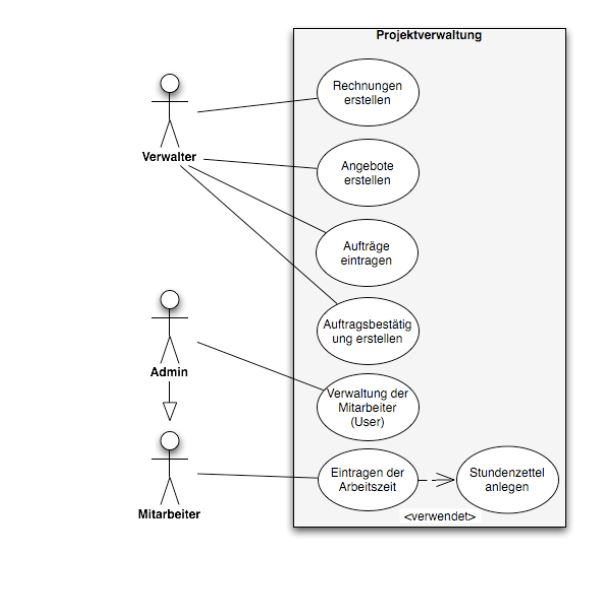
\includegraphics[scale=0.8]{Graphics/Anwendungsdiagram.jpg} 
\captionof{figure}{Beispiel eines Anwendungsfalldiagramms in UML}



Quelle : DVZ datenverarbeitungszentrum mecklenburg-vorpommern gmbh

\label{fig2}


\end{figure}
\end{center}
\newpage
Anwendungsfalldiagramme weisen jedoch den Nachteil auf, dass keine Reihenfolge bei der Bearbeitung der Anwendungsfälle abgebildet werden kann. Es wird somit nicht deutlich, welcher Anwendungsfall vor einem anderen durchgeführt werden muss. Allerdings kann diese Reihenfolge beispielsweise durch andere Methoden der UML, wie das Aktivitätsdiagramm, kompensiert werden. Zudem muss jeder Anwendungsfall anhand einer Beschreibung dokumentiert werden. Hierbei bestehen jedoch keine Vorgaben, weshalb sich Inkonsistenzen und Redundanzen ergeben können. Darüber hinaus kann nicht sichergestellt werden, dass Dritte die Dokumentation auch verstehen. Daher sollte auf Vorlagen, die nicht offiziell zum Standard der UML gehören, zurückgegriffen werden.\\
\\
\newpage
Das Klassendiagramm (Class Diagram) eignet sich zur Darstellung von Klassenstrukturen innerhalb eines IKS. Klassendiagramme können nicht direkt für die Geschäftsprozessmodellierung verwendet werden. Stattdessen handelt es sich eine statische Darstellung von Klassen, Objekten und deren Beziehungen untereinander. Klassendiagramme beschreiben jedoch nur, dass eine Interaktion besteht; wie diese ausgestaltet ist kann jedoch nicht dargestellt werden.\\

\begin{center}
\begin{figure}[h]
   
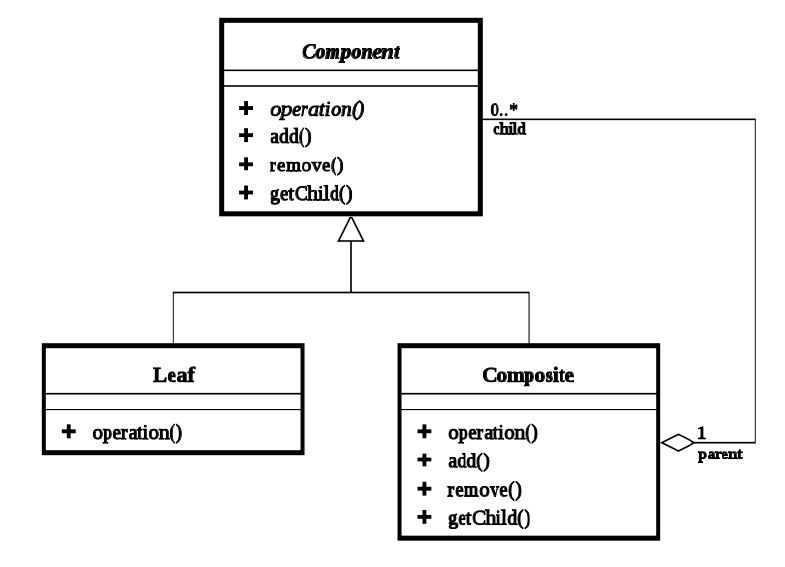
\includegraphics[scale=0.7]{Graphics/Klassendiagram.jpg} 
\captionof{figure}{Beispiel eines Klassendiagramms in UML}



Quelle : DVZ datenverarbeitungszentrum mecklenburg-vorpommern gmbh

\label{fig3}


\end{figure}
\end{center}
\newpage
Das Aktivitätsdiagramm oder auch Ablaufdiagramm (Activity Diagram) wird zur Darstellung von Abläufen verwendet. Im Mittelpunkt steht dabei die Visualisierung paralleler Abläufe. Aus diesem Grund eignet sich dieser Diagrammtyp in einem besonders hohen Maße zur Abbildung von Geschäftsprozessen, da diese zumeist Parallelitäten vorweisen. Aktivitätsdiagramme sind darüber hinaus zur Modellierung von Workflows und zur Verfeinerung von Anwendungsfällen geeignet. Des Weiteren sind Aktivitätsdiagramme in der Lage unterschiedliche Detaillierungsgrade wiederzugeben. So ist es unter anderem möglich ein anwendungsfallübergreifendes Diagramm zu erzeugen und anschließend die darin enthaltenen Anwendungen einzeln zu modellieren.\\ \\

\begin{center}
\begin{figure}[h]
   

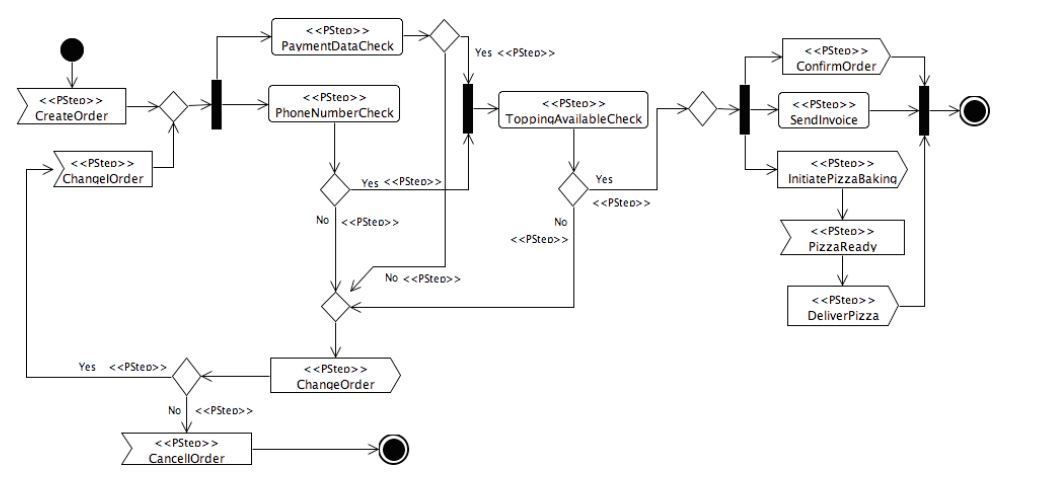
\includegraphics[scale= 0.65]{Graphics/activitydiagram.jpg} 
\captionof{figure}{Beispiel eines Aktivitätsdiagramm in UML}



Quelle : DVZ datenverarbeitungszentrum mecklenburg-vorpommern gmbh

\label{fig4}


\end{figure}
\end{center}

\newpage
\subsection{UML-Diagramme: Eine Übersicht}
Die folgende Übersicht zeigt übergeordnete Kategorien und Anwendungsmöglichkeiten der einzelnen Diagrammtypen in Kurzform. Wenn Sie ein modellorientiertes Software-System, einen Anwendungsfall in der Wirtschaft o. Ä. visuell darstellen wollen, sollten Sie laut Empfehlung der UML-Task-Force vorher einen der UML-Diagrammtypen wählen. Erst dann lohnt es sich, eines der vielen UML-Tools zu wählen, da diese häufig eine gewisse Methode vorschreiben. Dann erstellen Sie das UML-Diagramm.\\
\begin{center}
\begin{figure}[h]
   

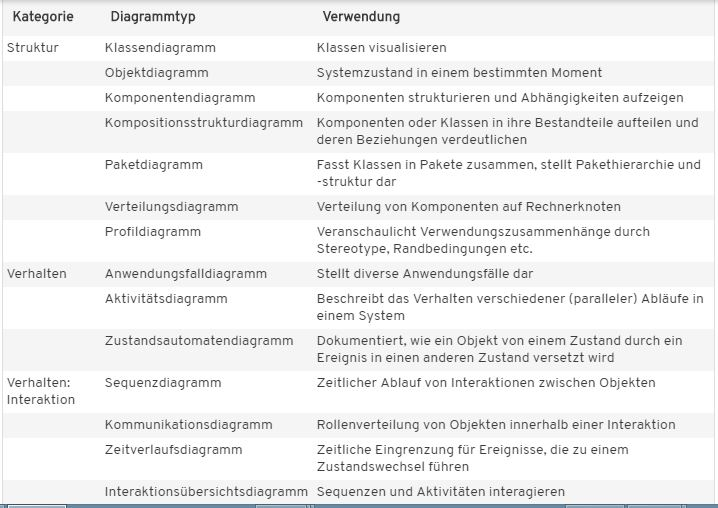
\includegraphics[scale=0.8]{Graphics/UMLdiagramme.jpg} 
\captionof{figure}{UML-Diagramme}

 Quelle : Ionos - Digital Guide 
 
\label{fig5}


\end{figure}
\end{center}
\newpage
\subsection{Vor- und Nachteile im Überblick}
UML ist heute eine der dominierenden Sprachen für die Modellierung von betrieblichen Anwendungs- bzw. Softwaresystemen. Der erste Kontakt zu UML besteht häufig darin, dass UML-Diagramme im Rahmen von Softwareprojekten zu erstellen, zu verstehen oder zu beurteilen sind. UML-Diagramme gelten als Standard bei objektorientierter Modellierung.\\

\begin{center}
\begin{figure}[h]
   

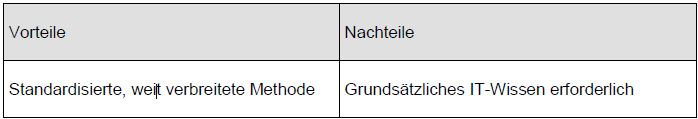
\includegraphics[scale=0.8]{Graphics/vornach.jpg}
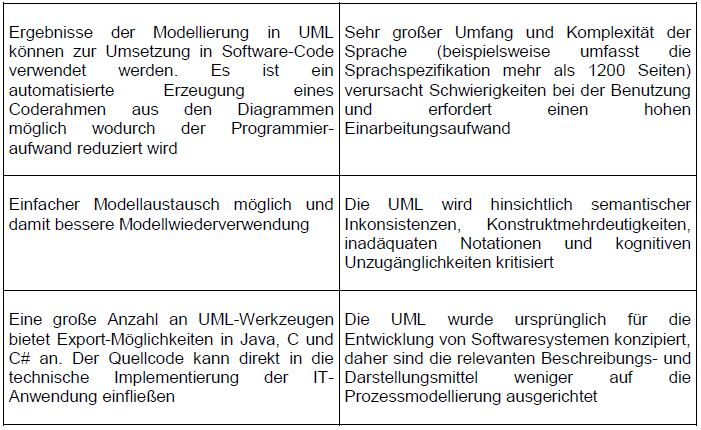
\includegraphics[scale=0.8]{Graphics/vornach2.jpg} 
\captionof{figure}{UML: Vor- und Nachteile }


Quelle : DVZ datenverarbeitungszentrum mecklenburg-vorpommern gmbh 

 
\label{fig6}


\end{figure}

\end{center}
\newpage
\section{MSC}
MSC ist eine vom ITU-T als Recommendation Z.120
standardisierte graphische Spezifikationssprache. Sie dient
zur Beschreibung des Kommunikationsverhaltens zwischen
Systemkomponenten und deren Umgebung. Die Kommunikation
wird durch den Austausch von Nachrichten (Messages)
spezifiziert.\\
Die MSC-Sprache hat sich aus den OSI Time Sequence
Diagrams zu einer vollst¨andigen graphischen Sprache
mit formaler Syntax und Semantik entwickelt.
Mit den Sequence Diagrams wurde eine Variante von MSC
in die UML integriert. Obwohl beide Sprachen auf den
gleichen Prinzipien beruhen, gibt es auf Grund der verschiedenen
Anwendungsbereiche unterschiedliche Sprachkonstrukte
und Unterschiede in der Darstellung. Durch eine
Kombination der Stärken von MSC und den Sequence
Diagrams bemüht man sich zur Zeit verstärkt um eine Harmonisierung der beiden Diagrammarten.\\
In diesem Abschnitt werden die wichtigsten Konstrukte der
MSC-Sprache an Hand von MSCs1 für das in der Einleitung zu dieser Abschnittreihe beschriebene Beispiel erläutert. Das Beispiel beschreibt einen Produktionsprozess, in dem eine Produktionszelle aus vier verschiedenen Einzelteilen vom Typ A, B, C und D zwei Produkte vom Typ AC und BDC herstellt.


\subsection{Basic-MSC}
Basic-MSC umfasst alle Sprachkonstrukte, die notwendig sind, um den Nachrichtenfluss zu spezifizieren. Diese
Sprachkonstrukte sind: Instanz, Message, Environment, Action, Timer-Start, Timeout, Timer-Stop, Create, Stop und
Condition.\\

\begin{center}
\begin{figure}[h]
   

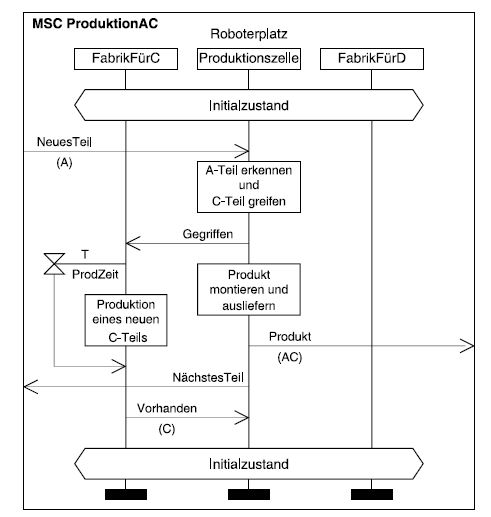
\includegraphics[scale=1]{Graphics/MSC1.jpg}

\captionof{figure}{Ein Basic-MSC }


Quelle : The Specification Languages MSC and SDL
Part 1: Message Sequence Chart (MSC) 

 
\label{fig7}


\end{figure}

\end{center}
\newpage
Ein Basic-MSC mit dem Namen ProduktionAC ist in
Abbildung 1.6 gezeigt. Es beschreibt die Produktion eines aus einem
A- und einem C-Teil zusammengesetzten Produkts.
Das MSC abstrahiert von den Details und zeigt nur den Informationsaustausch
zwischen den drei Hauptkomponenten
des Produktionsprozesses: Der Produktionszelle und den
zwei Fabriken für C- und D-Teile.
\\
Der Produktionsprozess befindet sich zu Beginn in seinem
Initialzustand: Das System ist initialisiert und Teile
der Typen C und D sind gefertigt, eingelagert und der
Produktionszelle zur Verfügung gestellt worden. Die Systemumgebung
übergibt ein A-Teil an die Produktionszelle.
Diese erkennt den Typ des Teils, greift das für die Produktion
notwendige C-Teil und meldet das Entfernen des
C-Teils vom Greifplatz an die Fabrik, die C-Teile herstellt.
Ein Produkt vom Typ AC wird gefertigt und dann
ausgegeben. Danach meldet die Produktionszelle die Bereitschaft
für die Bearbeitung des nächsten A- oder B-Teils
an die Systemumgebung. Parallel zu den Aktionen der Produktionszelle
wird ein neues C-Teil produziert und zur
Verfügung gestellt.\\
\subsubsection{Instanz und Message}
Die wichtigsten Sprachkonstrukte von Basic-MSC sind Instanz
und Message. Instanzen sind Komponenten, die untereinander
oder mit der Systemumgebung asynchron Messages
austauschen können.\\
In der graphischen Form werden Instanzen als vertikale
Linien oder alternativ als Säulen dargestellt. Innerhalb
des Instanzkopfes wird der Instanzname spezifiziert,
zus¨atzlich kann ein Typ angegeben werden (z.B. Instanz
Produktionszelle vom Typ Roboterplatz in
Bild 1). Das Ende einer Instanz kann durch ein Instanz-
Ende-Symbol beschrieben werden. Ein Instanz-Ende
bedeutet nicht, dass die Instanz gestoppt ist, sondern lediglich
dass in dem MSC keine weiteren Ereignisse für die
Instanz beschrieben werden.\\
Messages werden durch Pfeile dargestellt. Diese Pfeile
k¨onnen horizontal oder geneigt sein, um den Zeitverlauf
anzuzeigen. Eine Message definiert zwei Ereignisse: Der
Pfeilanfang beschreibt das Senden und die Pfeilspitze bezeichnet
die Verarbeitung einer Message. Die Beschriftung
einer Message besteht aus ihrem Namen und optionalen
Message-Parametern, die in Klammern angegeben werden
m¨ussen (z. B. Message NeuesTeil mit dem Parameter A
in Abbildung 1.6).\\
Entlang jeder Instanzachse wird eine Totalordnung der spezifizierten
Message-Sende- und Message-Verarbeitungsereignisse
angenommen. Ereignisse auf verschiedenen Instanzachsen
werden durch Message-Kommunikation partiell
geordnet, da eine Message zuerst gesendet werden muss,
bevor sie verarbeitet werden kann.
\subsubsection{Environment}
Die Diagrammfläche eines MSC wird durch einen rechteckigen
Rahmen begrenzt. Der Diagrammrahmen definiert
die Systemumgebung und heißt Environment. Messages,
die aus der Systemumgebung kommen oder an die Systemumgebung
gesendet werden, beginnen und enden auf
dem Environment (z.B. die Messages NeuesTeil und
Produkt in Bild 1). Im Gegensatz zur Totalordnung entlang
der Instanzachsen ist für Sende- und Verarbeitungsereignisse
auf dem Environment keine Ordnung definiert.\\
\subsubsection{Action}
Zusä¨atzlich zur Message-Kommunikation können Aktionen
von Instanzen in Form von Actions spezifiziert werden.
Eine Action wird durch ein Rechtecksymbol dargestellt, das
beliebigen Text enthalten kann (z. B. Action ,Produkt
montieren und ausliefern‘ in Abbildung 1.6).\\
\subsubsection{Timer}
Zur Beschreibung von Timern bietet MSC die Sprachkonstrukte
Timer-Start, Timeout und Timer-Stop an. Timer-Start
spezifiziert das Setzen, Timeout den Ablauf und Timer-Stop das Zur¨ucksetzen eines Timers. In MSC ist ein Timer
immer einer Instanz zugeordnet. Die graphischen Timer-Symbole sind daher immer mit der dem Timer zugeordneten
Instanz verbunden.\\

Ein Timer-Start wird durch ein mit der Instanzachse
verbundenes Sanduhr-Symbol dargestellt. Ein zugehöriges
Timeout wird durch einen Pfeil beschrieben, der am
Sanduhr-Symbol beginnt und auf der Instanzachse endet.
Ein Timer-Stop wird durch ein mit der Instanzachse verbundenes
Kreuz beschrieben. Ein Timersymbol wird mit
dem Timernamen und optional mit Timer-Parametern versehen.
Ein Timer-Start und das zugeh¨orige Timeout werden
in Bild Abbildung 1.6 verwendet, um die Produktionszeit für ein Teil des
Typs C zu modellieren. Der Timer hat den Namen T und
den Parameter Prodzeit, der die Laufzeit des Timers
spezifiziert.\\
\subsubsection{Condition}
Eine Condition beschreibt einen Zustand, der sich auf
eine Menge der im MSC enthaltenen Instanzen bezieht.
Graphisch werden Conditions durch Sechsecke dargestellt,
die die Instanzen, auf die sich die Condition bezieht,
¨uberdecken. Conditions werden zur Beschreibung von
wichtigen Systemzuständen benutzt. In Bild Abbildung 1.6 befinden sich
zwei Conditions, die beide den globalen Systemzustand
Initialzustand beschreiben.\\
\subsubsection{Create und Stop}
Die MSC-Sprache enthält die Konstrukte Create und Stop
für die dynamische Erzeugung und Terminierung von Instanzen.
Ein Create wird durch einen gestrichelten Pfeil
mit optionalen Parametern beschrieben. Ein Create-Pfeil
beginnt an der Erzeuger-Instanz und endet am Kopf der erzeugten
Instanz. Eine Instanz kann sich selbst durch eine
Stop-Aktion terminieren. Ein Stop wird graphisch durch ein
Kreuz am Ende der Instanzachse spezifiziert.\\

\subsection{Strukturelle Sprachkonstrukte}
Strukturelle MSC-Sprachkonstrukte bezeichnen Sprachelemente,
die über die Beschreibung des reinen Messageflusses
hinausgehen. Mit ihnen lassen sich MSCs und
MSC-Teile zu komplexeren Abläufen kombinieren (Inline-
Expressions und High-Level-MSC), MSC-Diagramme in
anderen MSC-Diagrammen wiederverwenden (References),
MSC-Instanzen verfeinern (Decomposition) und allgemeine
Ereignisstrukturen für Instanzen definieren (Coregion und
General Ordering). Aus Platzgründen kann im Rahmen
dieses Artikels nur auf Inline-Expressions, References und
High-Level-MSC (HMSC) eingegangen werden.\\

\begin{center}
\begin{figure}[h]
   

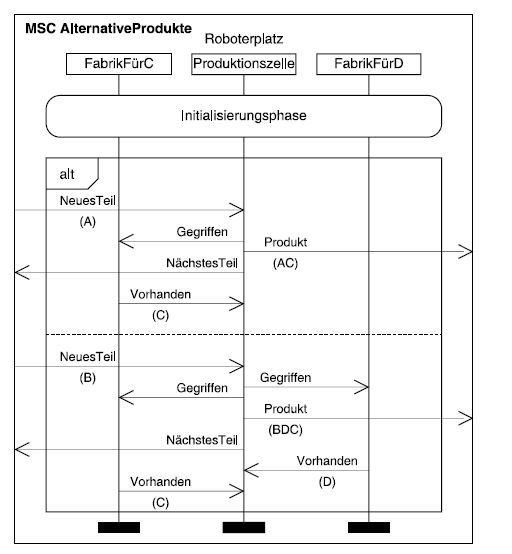
\includegraphics[scale=1]{Graphics/MSCmit.jpg}

\captionof{figure}{MSC mit strukturellen Sprachkonstrukten }


Quelle : The Specification Languages MSC and SDL
Part 1: Message Sequence Chart (MSC) 

 
\label{fig8}


\end{figure}

\end{center}
\newpage
\subsubsection{Inline-Expressions}
Mit Inline-Expressions können Teilabl¨aufe, die innerhalb
eines MSC-Diagramms spezifiziert worden sind, zu komplexeren
Abläufen kombiniert werden. Für die Kombination
bietet MSC die Operatoren alt, par, loop, opt und exc an. Sie erlauben es, die Wiederholung von Teilabläufen
(loop-Operator), alternative Teilabl¨aufe (alt-Operator), die
parallele Komposition von Teilabläufen (par-Operator), optionale
Teilabläufe (opt-Operator) und Ausnahmen in Form
von Teilabläufen (exc-Operator) zu spezifizieren. Graphisch
werden Inline-Expressions als Rechtecke mit gestrichelten
Linien als Separatoren f¨ur Teilabläufe dargestellt. Der Operator
wird in der linken oberen Ecke spezifiziert.
Eine Inline-Expression mit einem alt-Operator befindet
sich in Abbildung 1.7 . Die alternativen Teilabläufe beschreiben
die Fertigung von Produkten der Typen AC und BDC in
Abhängigkeit des von der Systemumgebung übergebenen
Basisteils (A oder B).\\
\subsubsection{References}
References ermöglichen es, MSCs in anderen MSCs wieder
zu verwenden. Eine Reference referenziert ein anderes
MSC über dessen Namen, d. h. eine Reference kann als
Platzhalter für das referenzierte MSC angesehen werden.
Graphisch werden References durch ein Rechteck mit abgerundeten
Ecken dargestellt. Eine Reference befindet sich
auch in Abbildung 1.7 . Sie referenziert ein MSC mit dem Namen
Initialisierungsphase, das die Initialisierung
des Produktionsprozesses beschreibt.\\
\subsection{High-Level-MSC}
High-Level-MSC (HMSC) erlaubt es, die Kombination von
MSCs in Form eines gerichteten Graphen zu beschreiben.
Die Knoten eines HMSC-Diagramms sind ein Anfangsknoten, Endknoten, Konnektoren, References und Conditions.
\\ In HMSC konzentriert man sich auf die Darstellung
der Kombination von MSC-Diagrammen und abstrahiert
von den Instanzen und dem Messagefluss. HMSCDiagramme
werden häufig auch Roadmaps genannt. Mit
ihnen lässt sich die sequentielle, parallele und alternative
Kombination von MSCs in einer sehr intuitiven Form beschreiben.\\

\begin{center}
\begin{figure}[h]
   

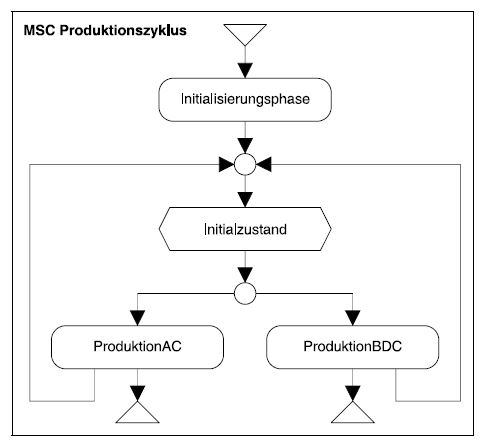
\includegraphics[scale=1]{Graphics/HMSC.jpg}

\captionof{figure}{Ein High-Level-MSC }


Quelle : The Specification Languages MSC and SDL
Part 1: Message Sequence Chart (MSC) 

 
\label{fig9}


\end{figure}

\end{center}
\newpage
Der HMSC in Abbildung 1.8 beschreibt die erwarteten AblÄufe
des Produktionsprozess-Beispiels: Nach der Initialisierungsphase
befindet sich der Produktionsprozess in seinem
Initialzustand. Im Initialzustand können entweder Produkte
vom Typ AC oder vom Typ BCD hergestellt werden. Nach
der Herstellung eines Produkts befindet sich der Produktionsprozess
wieder im Initialzustand und ein neues Produkt
kann gefertigt werden, oder der Produktionsprozess endet.

\subsection{Weitere Sprachkonstrukte}
In diesem Artikel konnten aus Platzgründen nur die
wichtigsten Elemente der MSC-Sprache vorgestellt werden.
Neben den genannten Konstrukten enthält MSC
noch einige weitergehende Konzepte, die MSC zu einer
vollständigen Spezifikationssprache machen: Die zu einer
Spezifikation gehörenden MSC-Diagramme können in
einem MSC-Dokument gesammelt und strukturiert werden.
MSC besitzt keine eigene Datensprache, aber eine
allgemeine Datenschnittstelle, die es erlaubt, Datenbeschreibungen
aus anderen Sprachen wie z. B. C, C++, SDL
oder Java zu benutzen. Zur Spezifikation von Realzeitanforderungen
können absolute Zeitpunkte und Zeitintervalle
in MSC-Diagrammen spezifiziert werden. Weiterhin wurden
UML-Konzepte zur objektorientierten Modellierung,
wie z. B. Control-Flow und Procedure-Calls, übernommen.

\section{Schluss}


\section{Referenz}




